\sectionalt{Introduction}

Lorem Ipsum is simply dummy text of the printing and typesetting industry. Lorem Ipsum has been the industry's standard dummy text ever since the 1500s, when an unknown printer took a galley of type and scrambled it to make a type specimen book \cite{gridftp}. It has survived not only five centuries, but also the leap into electronic typesetting, remaining essentially unchanged. It was popularised in the 1960s with the release of Letraset sheets containing Lorem Ipsum passages, and more recently with desktop publishing software like Aldus PageMaker including versions of Lorem Ipsum.
\begin{enumerate}
  \item
  List item 1 that tabulates the information
  \item
  Second list item
  \item
  Another list item
  \item
  last list item
\end{enumerate}

Contrary to popular belief, Lorem Ipsum is not simply random text. It has roots in a piece of classical Latin literature from 45 BC, making it over 2000 years old. Richard McClintock, a Latin professor at Hampden-Sydney College in Virginia, looked up one of the more obscure Latin words, consectetur, from a Lorem Ipsum passage, and going through the cites of the word in classical literature, discovered the undoubtable source. Lorem Ipsum comes from sections 1.10.32 and 1.10.33 of "de Finibus Bonorum et Malorum" (The Extremes of Good and Evil) by Cicero, written in 45 BC. This book is a treatise on the theory of ethics, very popular during the Renaissance. The first line of Lorem Ipsum, "Lorem ipsum dolor sit amet..", comes from a line in section 1.10.32.

The standard chunk of Lorem Ipsum used since the 1500s is reproduced below for those interested. Sections 1.10.32 and 1.10.33 from "de Finibus Bonorum et Malorum" by Cicero are also reproduced in their exact original form, accompanied by English versions from the 1914 translation by H. Rackham.

\begin{figure}[ht]
  \begin{center}
    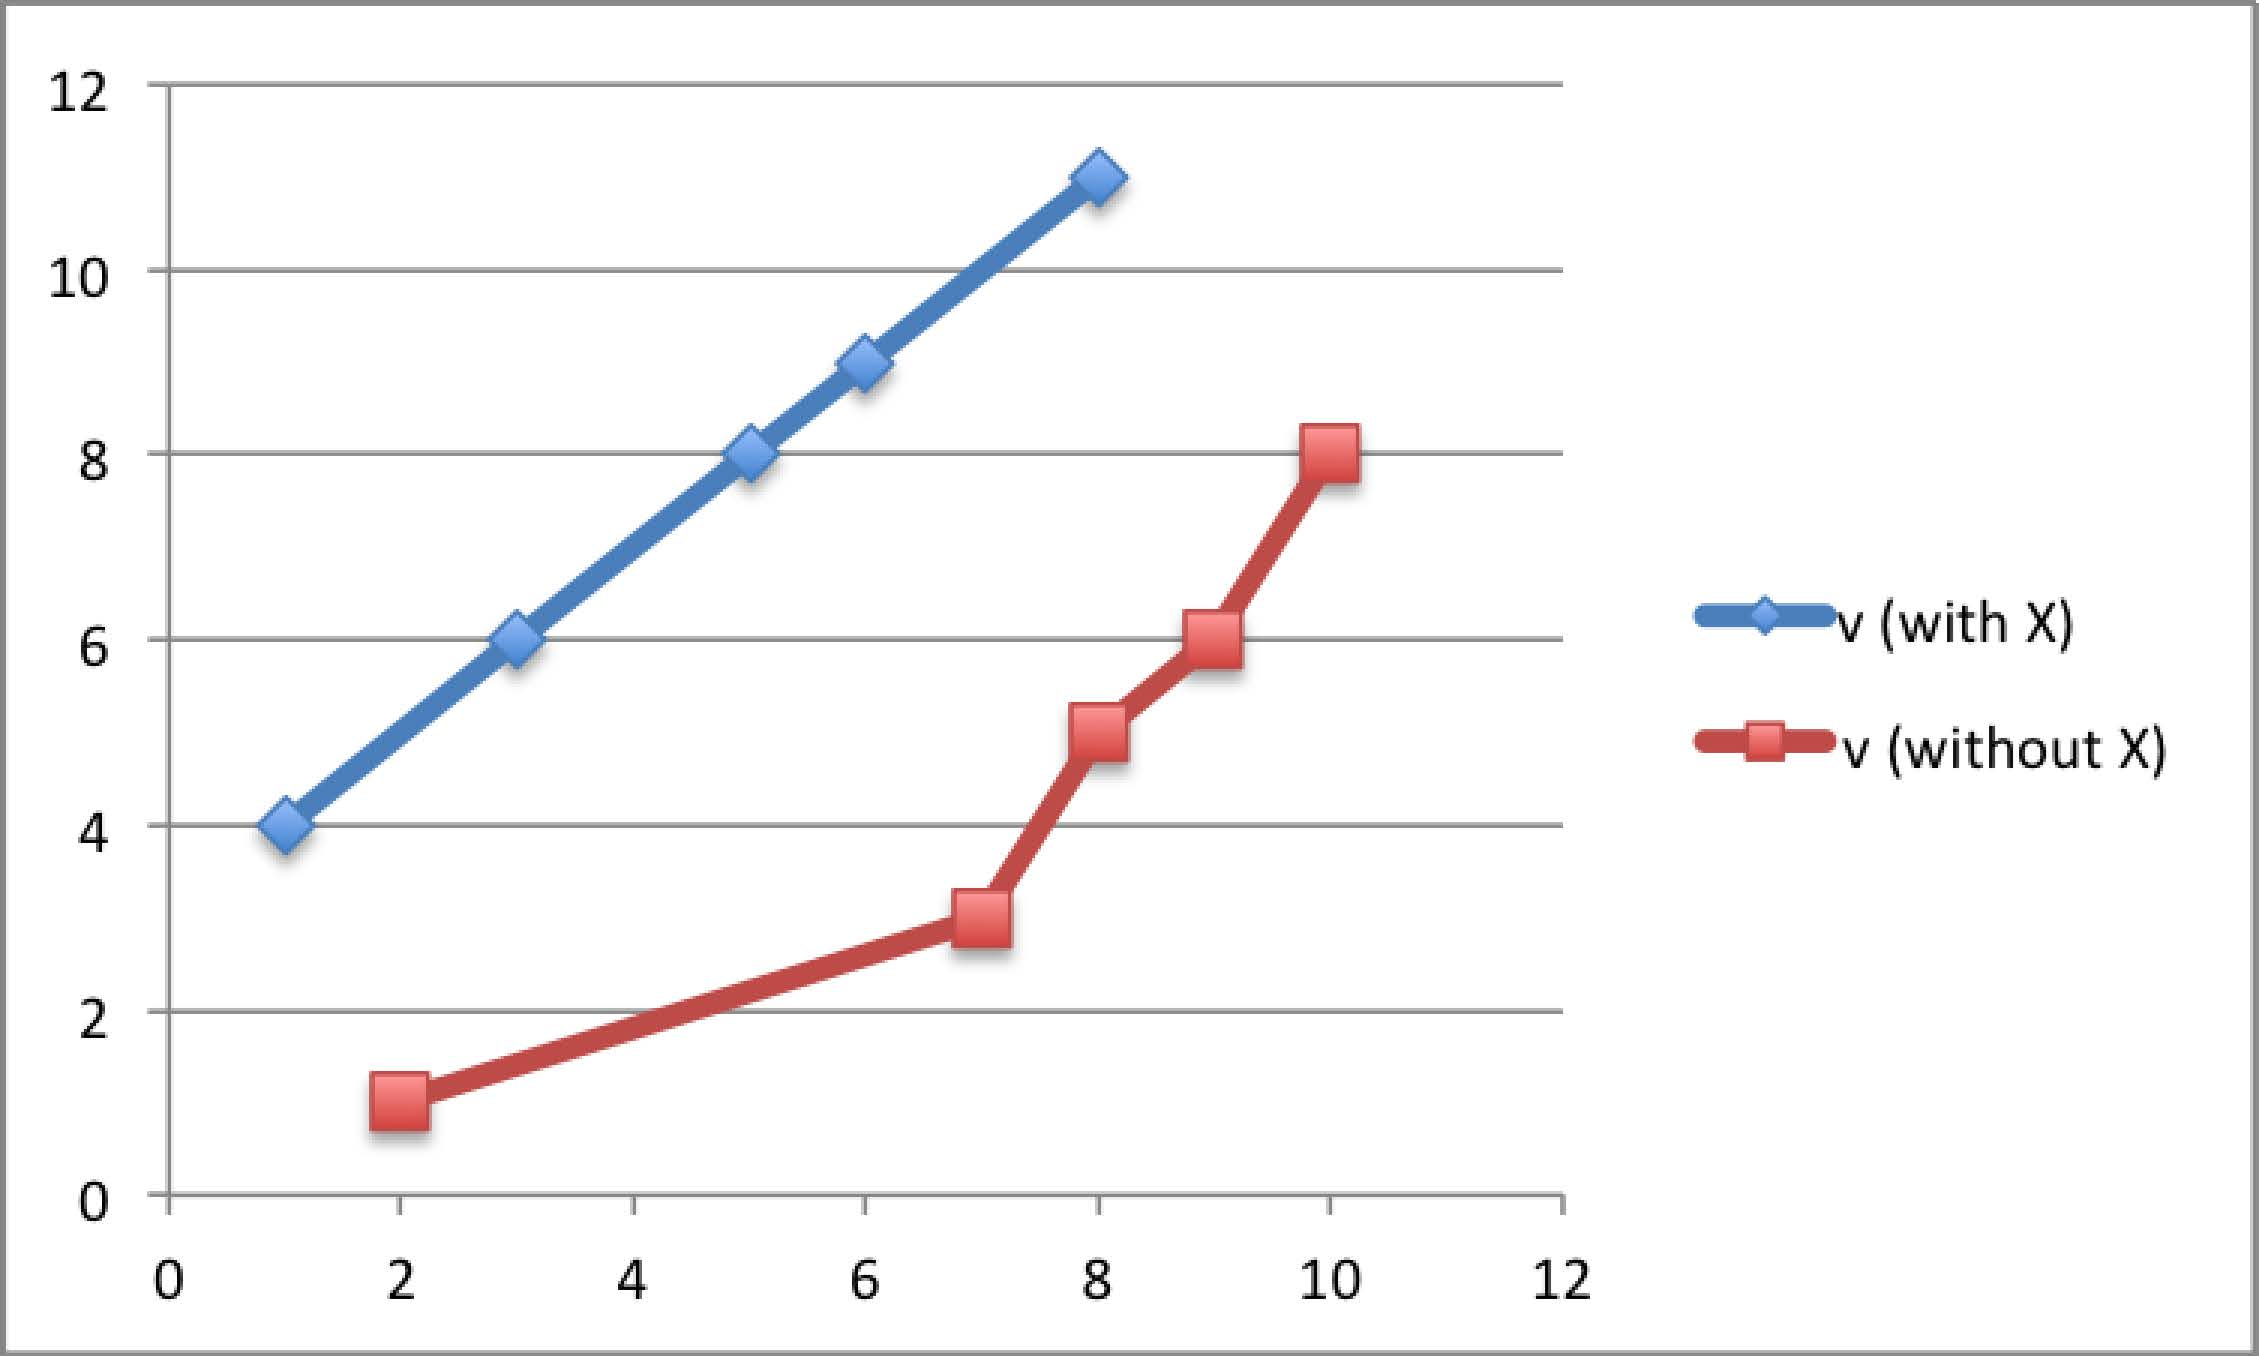
\includegraphics[scale=0.75]{RD}
    \caption{A sample graph image}
  \end{center}
\end{figure}

\subsection{Subfig test}

\begin{figure}[ht]
  \centering
  \subfloat[First fig.]{
    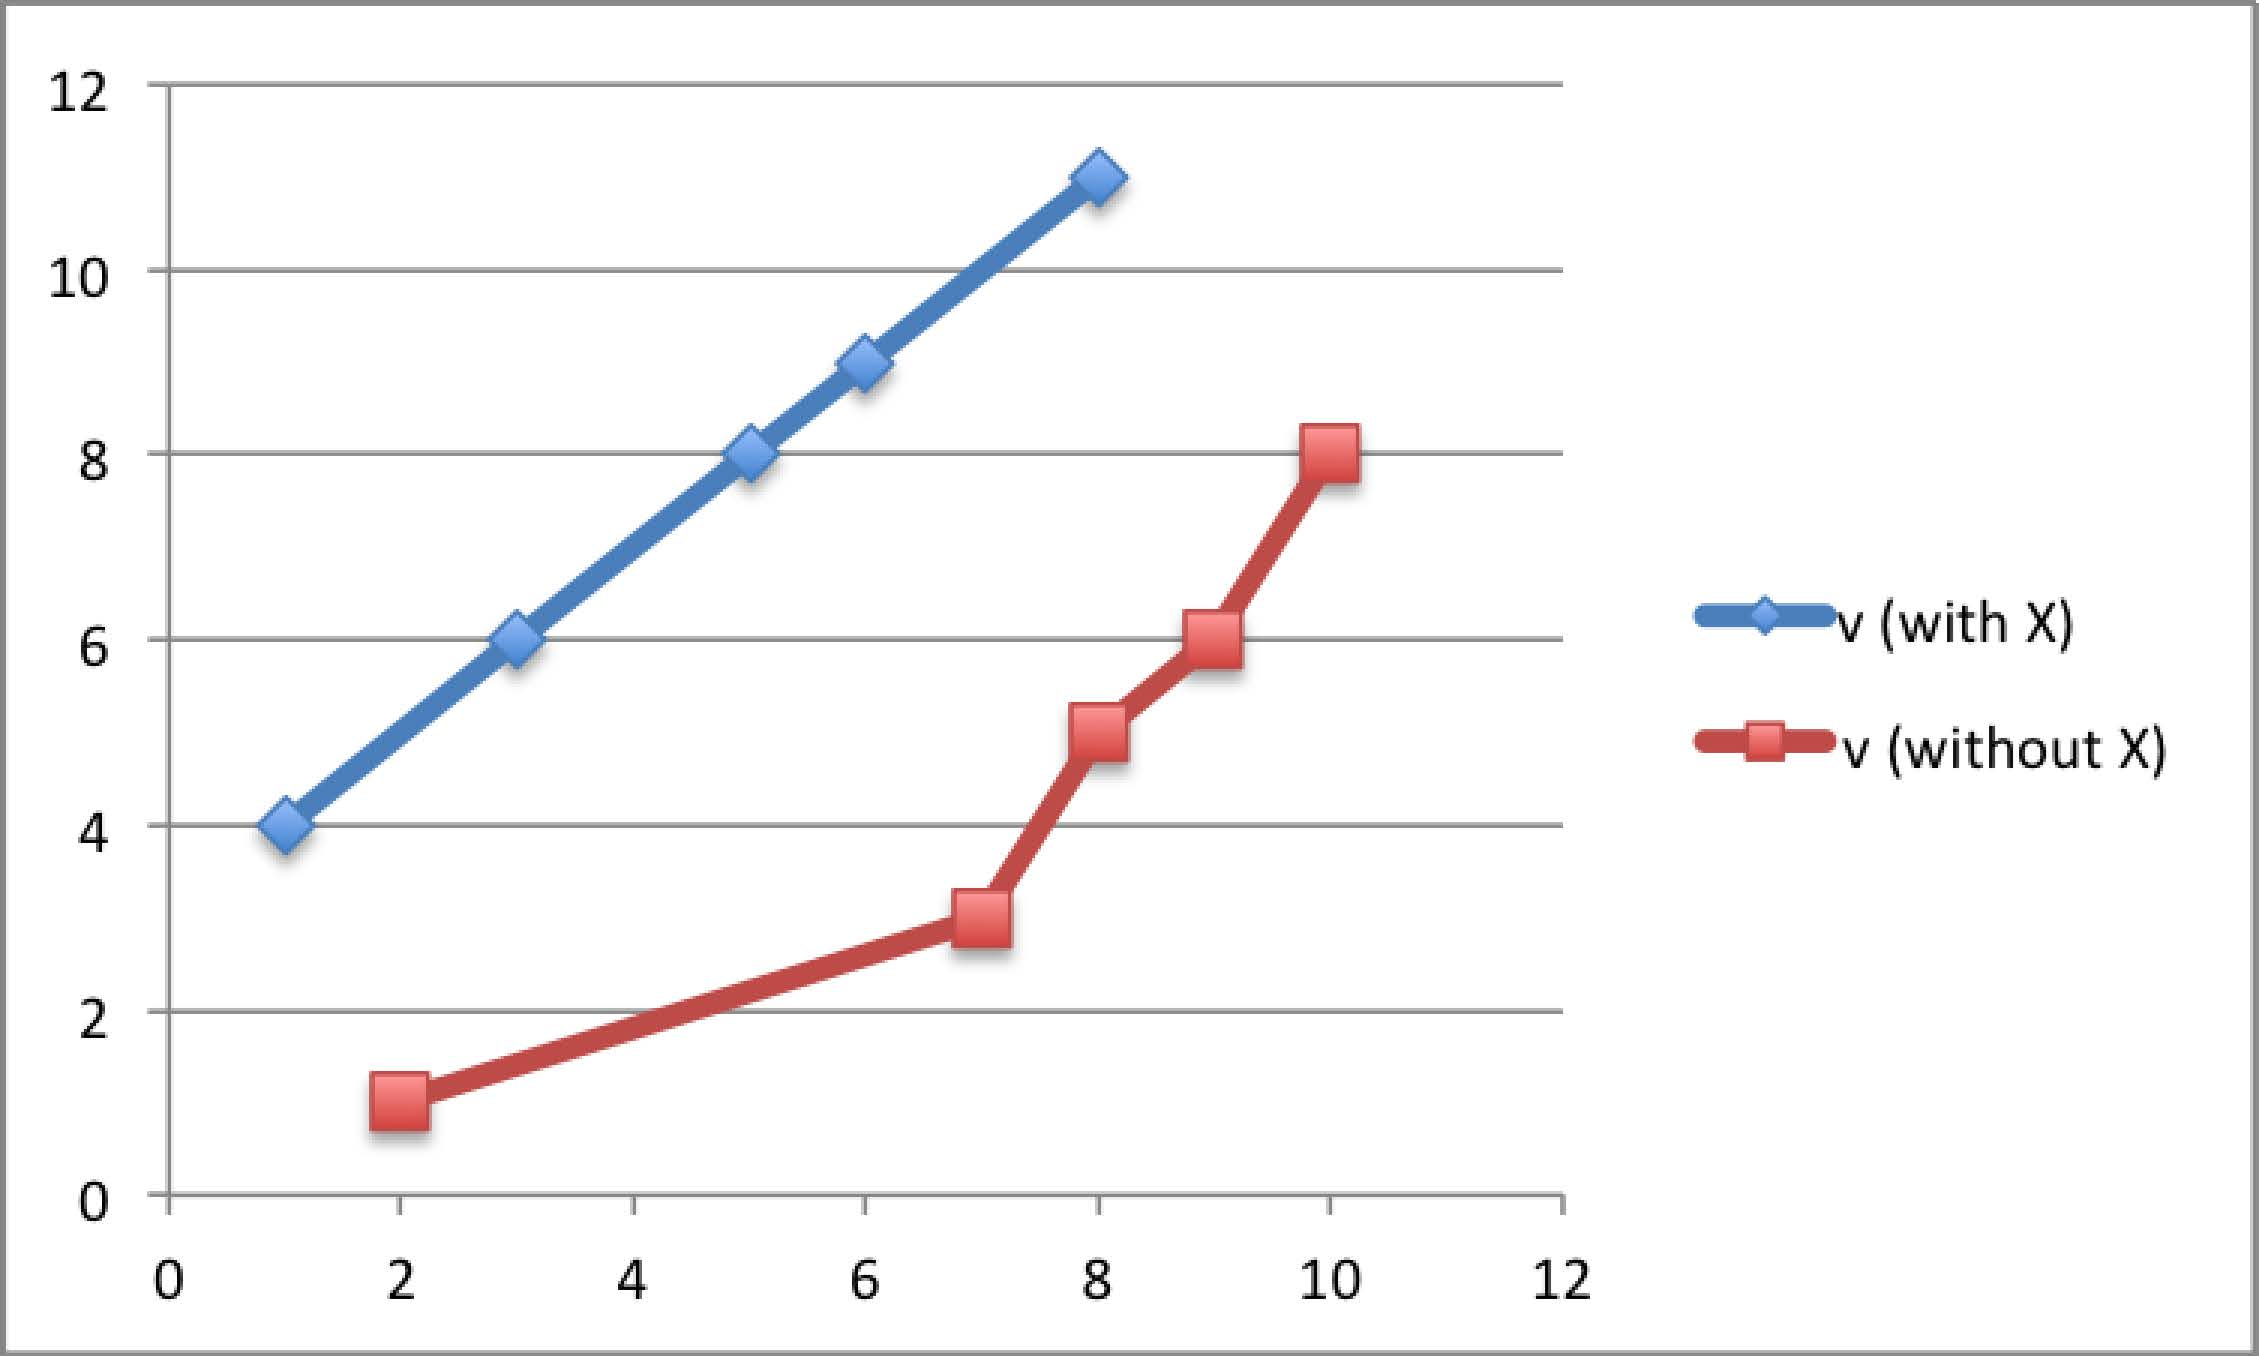
\includegraphics[width=0.45\columnwidth]{RD} \label{fig:two-figs:v1}
  }
  \subfloat[Second fig.]{
    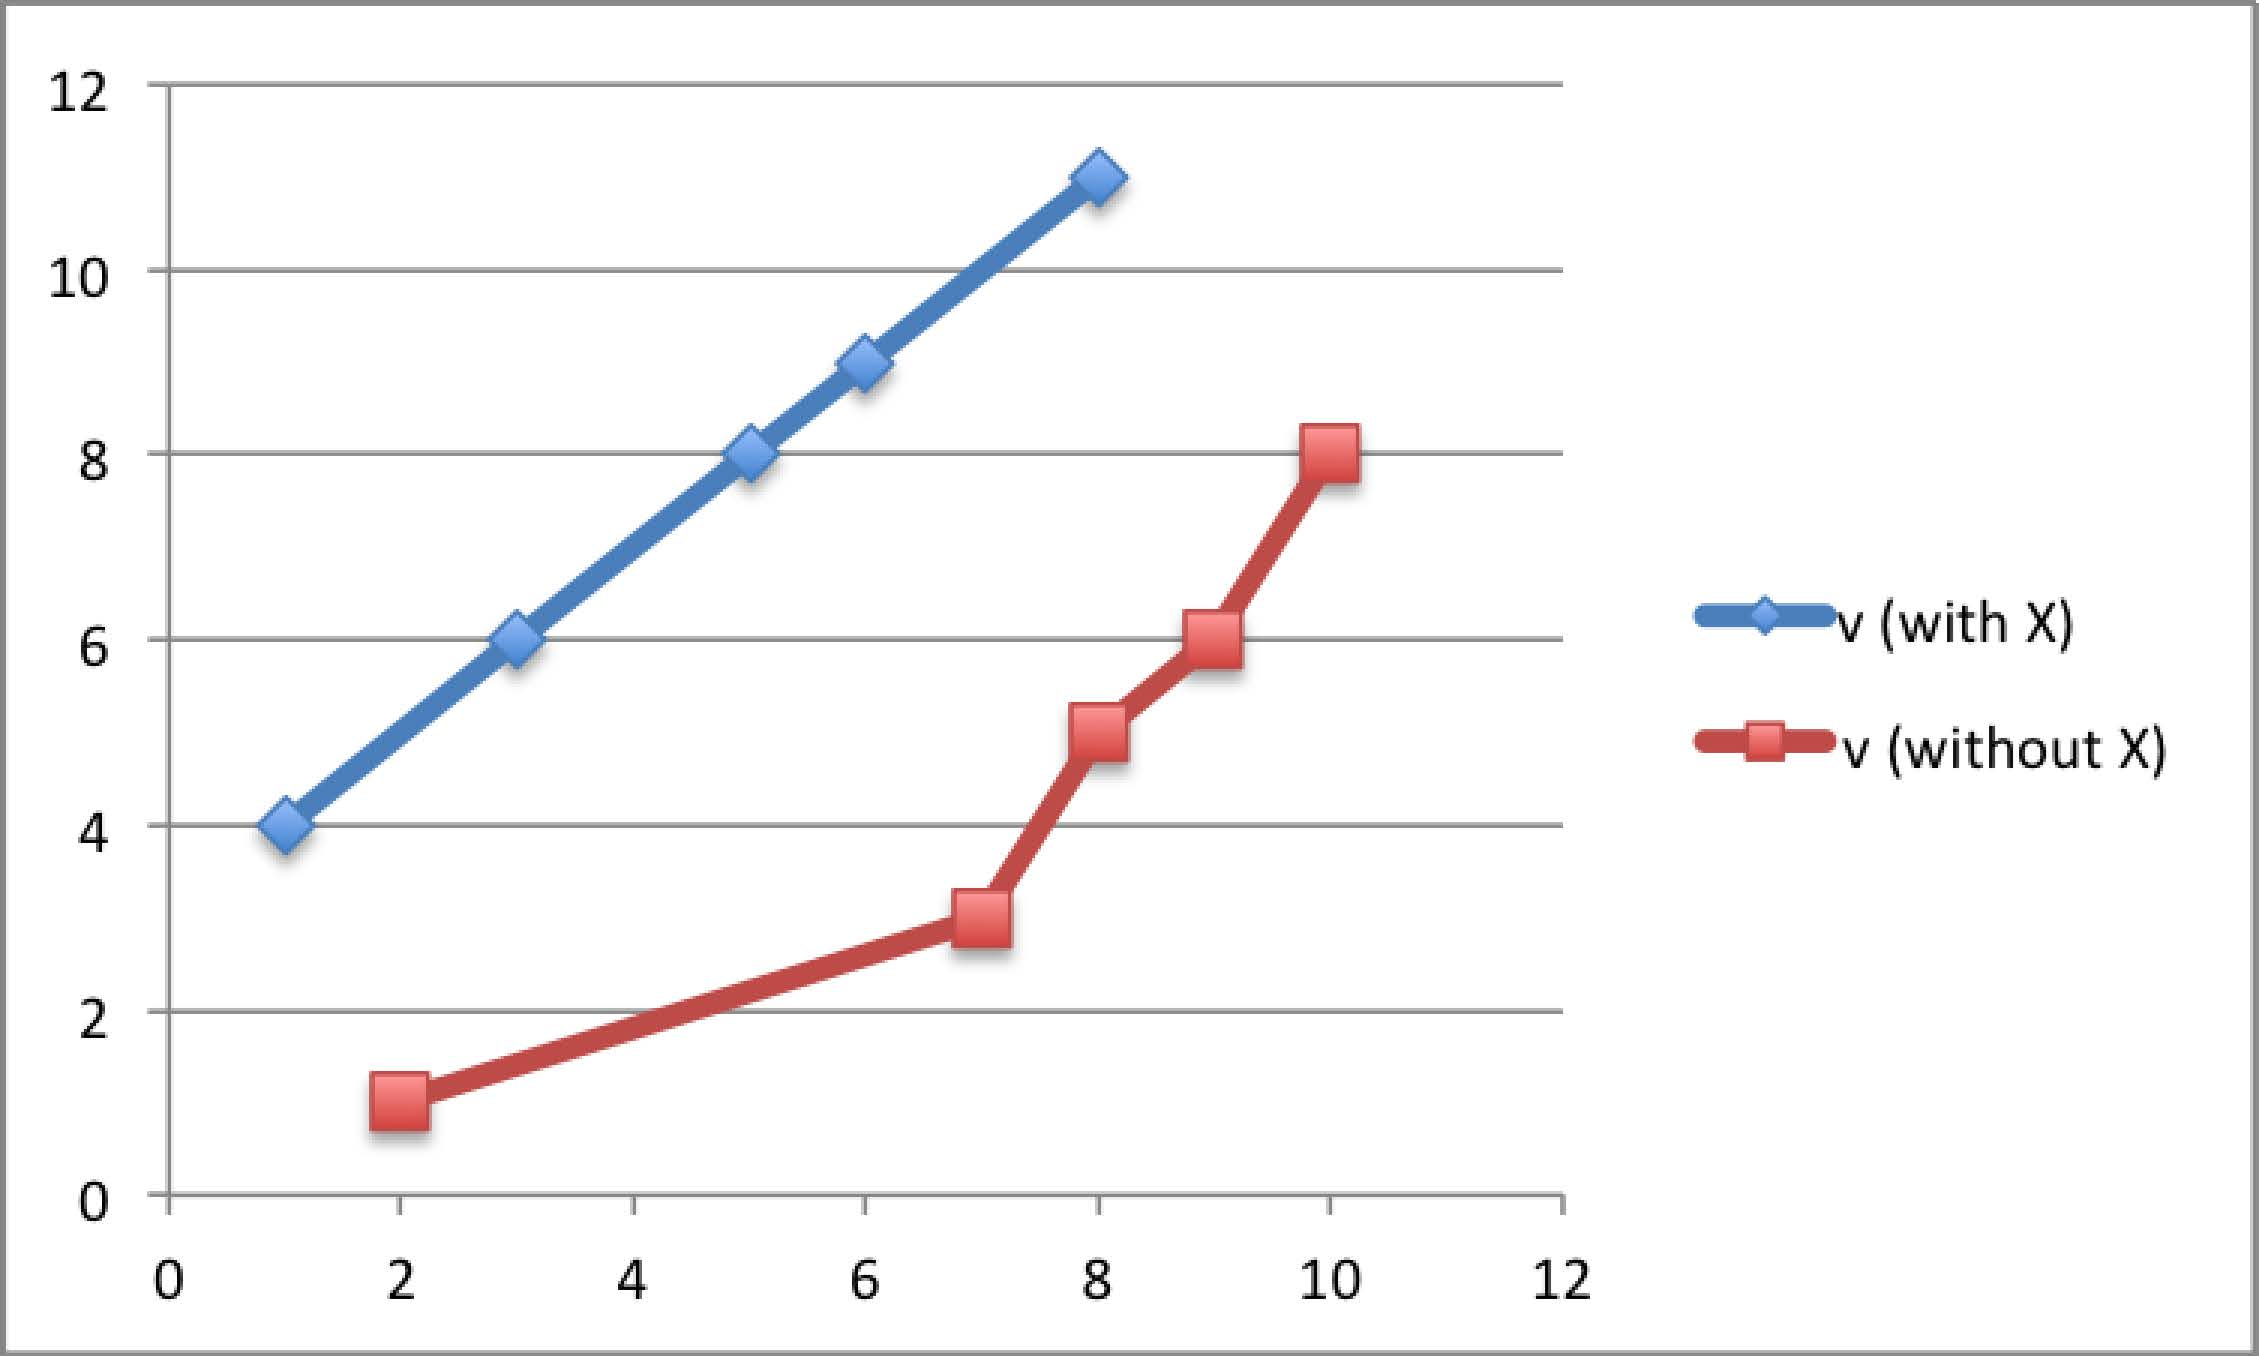
\includegraphics[width=0.45\columnwidth]{RD}
  }
  \caption{A sample of two sub figures. The two different figures are combines by the \texttt{subfloat} package. This figure has an extreme long caption for verifying whether the hanging paragraph of the single-spacing caption works. \label{fig:two-figs}}
\end{figure}

Try to ref \autoref{fig:two-figs}, and \autoref{fig:two-figs:v1}.

\subsection{Formulation test}
Test the following formulation. No comma should be used if there are only two equations:
\begin{subequations}
  \renewcommand{\theequation}
  {\theparentequation-\arabic{equation}}
  \begin{align}
    \frac{\partial \mathcal{L}(\mathbf{w},~b)}{\partial \mathbf{w}} &= \mathbf{w} + C \sum\limits_i\frac{\partial \ell_i}{\partial \mathbf{w}} \label{fml:eq1:partialW}\\
    \mathand~\frac{\partial \mathcal{L}(\mathbf{w},~b)}{\partial b} &= C \sum\limits_i\frac{\partial \ell_i}{\partial b}, \label{fml:eq1:partialb}
  \end{align}
\end{subequations}
where the gradients are used in support vector machine.

However, when there are more than 2 equations, commas should be used:
\begin{equation} \label{fml:ptl:robust}
  \begin{aligned}
    \argmin\limits_{\Theta} & \frac{1}{N_{tr}} \sum_{i=1}^{N_{tr}} \mathcal{L}\left(\mathbf{d}_{HF}^{(i)}, \mathbf{d}_{LF}^{(i)}\right) + \frac{\lambda/2}{N_{tr}} \sum_{i=1}^{N_{tr}} \mathcal{R}\left(\mathbf{d}_{HF}^{(i)}\right) + \frac{\lambda/2}{N_{ts}} \sum_{i=1}^{N_{ts}} \mathcal{R}\left(\mathbf{d}^{(i)}\right), \\
    &\mathcal{L} \left( \mathbf{d}_{HF}, \mathbf{d}_{LF} \right) = \left\lVert \mathcal{D}_{\Theta}\left( \mathbf{d}_{HF} \right) - \mathbf{d}_{LF} \right\rVert^2_2, \\
    \mathand~&\mathcal{R} \left( \mathbf{d} \right) = \left\lVert \mathcal{D}_{\Theta}\left( \mathbf{d} \right) - \Psi\left(\mathcal{D}_{\Theta}\left( \mathbf{d} \right)\right) \right\rVert^2_2.
  \end{aligned}
\end{equation}

Try to refer the equations like this: \eqref{fml:eq1:partialb}.

\subsection{Table test}

The title of the table should appear on the top of the table.

\begin{table}[tbp]
  \centering
  \caption{Example table.\label{tbl:res-accu}}
  \begin{tabularx}{0.6\textwidth}{|c|X<\centering|X<\centering|X<\centering|X<\centering|}
    \hline
    & Col 1 & Col 2 & Col 3 & Col 4 \\ \hline
    $\mathcal{L}_{\mathrm{a}}$ & $1$ & $2$ & $3$ & $4$ \\ \hline
    $\mathcal{L}_{\mathrm{b}}$ & $5$ & $6$ & $7$ & $8$ \\ \hline
  \end{tabularx}
\end{table}

\subsection{A Sample subsection}
It is a long established fact that a reader will be distracted by the readable content of a page when looking at its layout. The point of using Lorem Ipsum is that it has a more-or-less normal distribution of letters, as opposed to using 'Content here, content here', making it look like readable English \cite{gass}. Many desktop publishing packages and web page editors now use Lorem Ipsum as their default model text, and a search for 'lorem ipsum' will uncover many web sites still in their infancy. Various versions have evolved over the years, sometimes by accident, sometimes on purpose (injected humour and the like).

\begin{figure}[ht]
  \label{hourglass}
  \begin{center}
    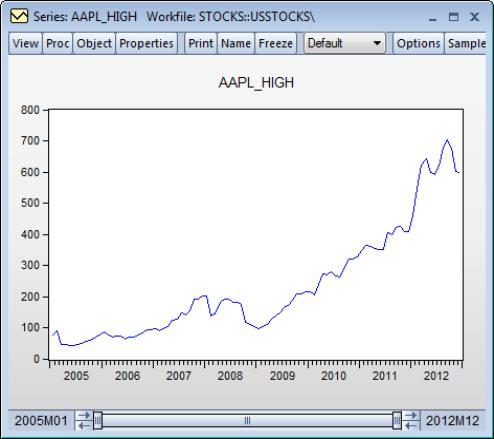
\includegraphics{graph}
    \caption{Another plot image}
  \end{center}
\end{figure}

\subsection{Another subsection} 
There are many variations of passages of Lorem Ipsum available, but the majority have suffered alteration in some form, by injected humour, or randomised words which don't look even slightly believable. If you are going to use a passage of Lorem Ipsum, you need to be sure there isn't anything embarrassing hidden in the middle of text. All the Lorem Ipsum generators on the Internet tend to repeat predefined chunks as necessary, making this the first true generator on the Internet. It uses a dictionary of over 200 Latin words, combined with a handful of model sentence structures, to generate Lorem Ipsum which looks reasonable. The generated Lorem Ipsum is therefore always free from repetition, injected humour, or non-characteristic words etc.
